\documentclass[../../main.tex]{subfiles}
\begin{document}
%
    To understand the mechanical properties of a cell, and, in turn, of the tissues the cell forms, we look to the cytoskeleton. Spanning the cell body, this active soft material, comprised and regulated by a vast number of proteins, confers structural stability to the cell. The cytoskeleton also plays a relevant role in a variety of cell processes such as motion, growth, division and phagocytosis.

    The cytoskeleton is composed of three major structural types of polymers. Each will be formed by the polymerization of a different kind of protein sub-unit and thus have a characteristic size and structure. The actin filaments are flexible helical polymers, made from the protein actin, that organise into a variety of linear bundles, two-dimensional networks, and three-dimensional gels. The microtubules are long, straight, hollow cylinders, much more rigid than the actin filaments. Finally, the intermediate filaments are rope-like fibres, smaller than the microtubules, constituting a very heterogeneous family \cite{albertsMolecularBiologyCell2015, hardinBeckerWorldCell2016}.
    
    Cytoskeleton organisation is also regulated by a myriad of accessory proteins. Among them we have cross-linkable proteins which are responsible for binding different filaments. They do so in different ways, depending on the type of protein. Some are only able to bind tightly apposed filaments, while others work over a wider range of angles \cite{coursonActinCrosslinkAssembly2010}. By regulating the density, activity and type of these accessory proteins, cells are able to create different structures without affecting the physical properties of the constituent elements. 
    
    Advances in biophysical techniques such as in fluorescence and atomic force microscopy, as well as in optical and magnetic tweezers have led to ever more precise studies on cell rheology \cite{mohammedInnovativeToolsMechanobiology2019, kollmannsbergerHighforceMagneticTweezers2007, masQuantitativeDeterminationOptical2013}. Different studies have noted a strong nonlinear increase in the elastic moduli of the network resulting from an increase in strain exerted \cite{linOriginsElasticityIntermediate2010, schopfererDesminVimentinIntermediate2009, gardelElasticBehaviorCrossLinked2004, piechockaMultiscaleStrainstiffeningSemiflexible2016, gardelStressDependentElasticityComposite2006, kangNonlinearElasticityStiff2009, koenderinkActiveBiopolymerNetwork2009}. After this regime of strain stiffening, an increase in compression levels leads to a reversible strain softening behaviour \cite{leeMolecularOriginStrain2010, chaudhuriReversibleStressSoftening2007}. Although this can be explained by the breaking of individual filaments, it is in the unbinding and, later, the re-binding of the cross-linkers that enable the elasticity of the network to recover so quickly. It has been shown that thermal energy is sufficient to entail cross-linker unbinding events, being responsible for the local rearrangement of the filaments and consequent energy dissipation \cite{lielegCytoskeletalPolymerNetworks2009, gardelStressDependentElasticityComposite2006, gardelElasticBehaviorCrossLinked2004, tharmannViscoelasticityIsotropicallyCrossLinked2007, semmrichNonlinearMechanicsEntangled2008, lielegTransientBindingDissipation2008, xuStrainHardeningStrain2011}. A nonlinear response in the form of negative normal stress has been also observed. This is quite unusual, with few materials sharing this characteristic, and those who do so, show a very weak response \cite{lin-gibsonElasticFlowInstability2004, montesiVorticityAlignmentNegative2004, ciferriLiquidCrystallinityPolymers1991}. In contrast, in bio-polymer networks, the negative normal stress can be comparable in magnitude to the applied shear \cite{contiCrossLinkedNetworksStiff2009}.

    As different experimental approaches are made, several models are devised with its usefulness usually tied to the timescales probed. The diverse behaviour of the bio-polymer network has led to a lack of consensus on a single, general description for the network. Contrasting often with its synthetic counterparts, this has made it an interesting case study in soft condensed matter physics. 
    
    We start \cref{ch: polDynamics} with a description of the main concepts behind Brownian Dynamics. We introduce the Langevin equation, used throughout this work to model the motion of the different particles and derive the fluctuation theorem. We make use of an established theory of the Gaussian chain to study the statistical properties of a single polymer chain with a focus on the equilibrium state and under shear. We do this in order to shed light on the intra-particle interactions and use it as a way to validate our code, since analytical solutions can often be found and then compared to our numerical results (\cref{fig: intra}).
%
\begin{comment}
    We start this work by describing the main concepts behind Brownian Dynamics. We will introduce the Langevin equation, used throughout this work to model the motion of the different particles and derive the fluctuation theorem.  
    
    In \cref{ch: polDynamics}, we make use of an established theory to study the statistical properties of a single polymer chain with a focus on the equilibrium state, as well as some results under shear conditions. We do this in order to shed light on the intra-particle interactions and use it as a way to validate our code, since analytical solutions can often be found and then compared to our numerical results (\cref{fig: intra}).

    In \cref{ch: Particle-Particle Aggregation}, we study the inter-particle interaction with a focus on the interaction potentials in simple \textbf{M}olecular \textbf{D}ynamics (MD) simulations. This enables us to model the cross-link proteins, to develop a suited interaction potential and at the same time introduce and test some concepts behind the numerical implementation of such a problem (\cref{fig: inter}). 
\end{comment} 
    
    In \cref{ch: Particle-Particle Aggregation}, we develop a suited interaction potential, which is an extension of the Lennard-Jones potential, to study the binding and unbinding of particles in a diluted system. This enables us to model the cross-link proteins and, at the same time, to introduce and test some concepts behind the numerical implementation of such a problem (\cref{fig: inter}). 
    
    Finally, in \cref{ch: CrosslinkNet}, we tie all this together and study the behaviour of a reticulated network based on the Gaussian chain and interacting through the potential introduced in \cref{ch: Particle-Particle Aggregation} (\cref{fig: reticulated}). By adding steric interactions between different chains, we aim at a more realistic representation of a chain in solution, avoiding unrealistic chain overlapping. 
    %
        \begin{figure}[h]
            \centering
            \begin{subfigure}[b]{0.328\textwidth}
                \centering
                \includegraphics[width=\textwidth]{Figures/intra.png}
                \caption{}
                \label{fig: intra}
            \end{subfigure}
            \hfill
            \begin{subfigure}[b]{0.328\textwidth}
                \centering
                \includegraphics[width=\textwidth]{Figures/inter.png}
                \caption{}
                \label{fig: inter}
            \end{subfigure}
            \begin{subfigure}[b]{0.328\textwidth}
                \centering
                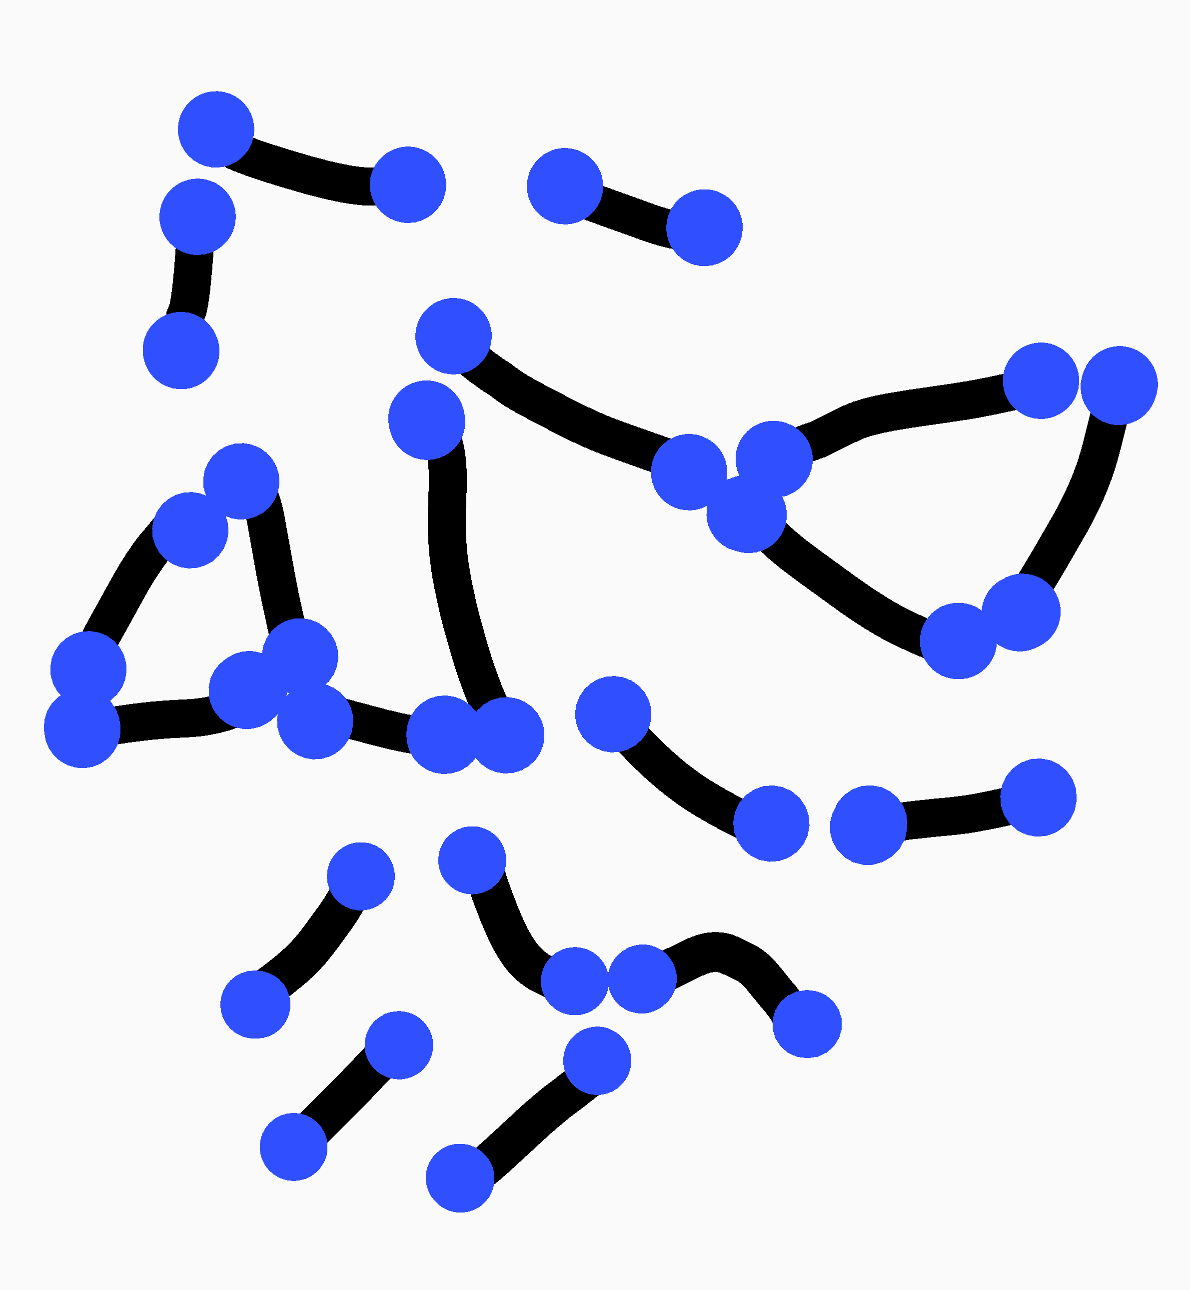
\includegraphics[width=\textwidth]{Figures/reticulated.png}
                \caption{}
                \label{fig: reticulated}
            \end{subfigure}
            \caption{Although slight modifications might be made to suit a specific case study, we present here a simple illustration of the three systems studied in this work. In \cref{fig: intra}, we have a bead-and-spring system with which we study intra-particle interactions; all particles interact over the same harmonic potential (\cref{eq: Gaussian Chain - Harmonic Spring Potential}). In \cref{fig: inter} we show particles enclosed in a box with periodic boundary conditions (\cref{app: PBC & MIC}) interacting via a pair potential; this system is used to study inter particle interactions and how they aggregate. Finally on \cref{fig: reticulated}, we have a cross-linked network; the blue particles represent cross-linkable proteins of a polymer chain that interact with those of the same kind via the pair potential described earlier (the chain represented in \cref{fig: intra} corresponds to the two blue ``dots" and the black line pair).}
        \end{figure}
        
\begin{comment}
    negative normal stress - network shrinks in the direction perpendicular to the applied shear stress
\end{comment}
    

%
\end{document}